\subsection{Project Track}
\textit{A graph is described by a set of nodes N (with an associated value) and a set of arcs (oriented pairs of nodes). The application should take a node value X, a starting node S and must return the number of occurrences in the graph of the input node X found in the graph during a bread first parallel search starting from the node S. The graph to be searched is assumed to be acyclic.}

\subsection{Graph Generation}
\label{sec:graph}
For the creation of the graphs has been developed an algorithm taking into account the objectives of the project and also the available storage and computational capabilities. The algorithm is based on the Erdős-Rényi model and has been implemented in C++.

To manage the graph is used a $map<key, value>$, in which the key is the node $id$ and the values are instances of the class $Node$. This class is provided of all the properties of a node:

\begin{itemize}
    \item $int$ $id$;
    \item $atomic$<$bool$> $visited$;
    \item $atomic$<$bool$> $discovered$;
    \item $vector$<$Node*$> $neighbors$.
\end{itemize}

The generation procedure requires in input the desired number of nodes \textit{no\_nodes} and a \textit{density}, that indicates the probability to have an edge between each distinct couple of nodes.  The generation starts filling a $map\{int, Node*\}$ with all the nodes of the graph. The next step is the connection between the nodes taking into account the direct and acyclic nature of the graph. So for each node the algorithm iterate on other nodes with larger ids and generates a random value between 0 and 1, if the number is below the density values a link is established. 

For testing the solutions has been created 3 graphs:
\begin{itemize}
    \item 10000 nodes and 0.02 of density;
    \item 10000 nodes and 0.5 of density;
    \item 10000 nodes and 0.8 of density.
\end{itemize}

\subsection{Problem Analysis}
\label{sec:Problem_Analysis}
The \textit{Breadth-First Search} (BFS) is a graph visit algorithm, that takes in input a graph $G(V, E)$ and a starter node $v\in V$. The $BFS$ starts initializing the frontier vector $F$ with the starter's neighbors $v$ and an empty one called next frontier $F'$. In the next phase start the visit of the nodes in $F$, and for each node three operations are performed: 1) marking the node as visited, 2) check if has the same value as the input one, and 3) his list of neighbors is scanned to update the next frontier $F'$. Every time a new node is discovered is marked as $discovered$ and added to $F'$. When the visit of the frontier $F$ ends, it gets cleared and swapped with $F'$. The frontier visit and the swapping step are repeated until the next frontier $F'$ is empty. 

\begin{figure}[htb!]
    \centering
    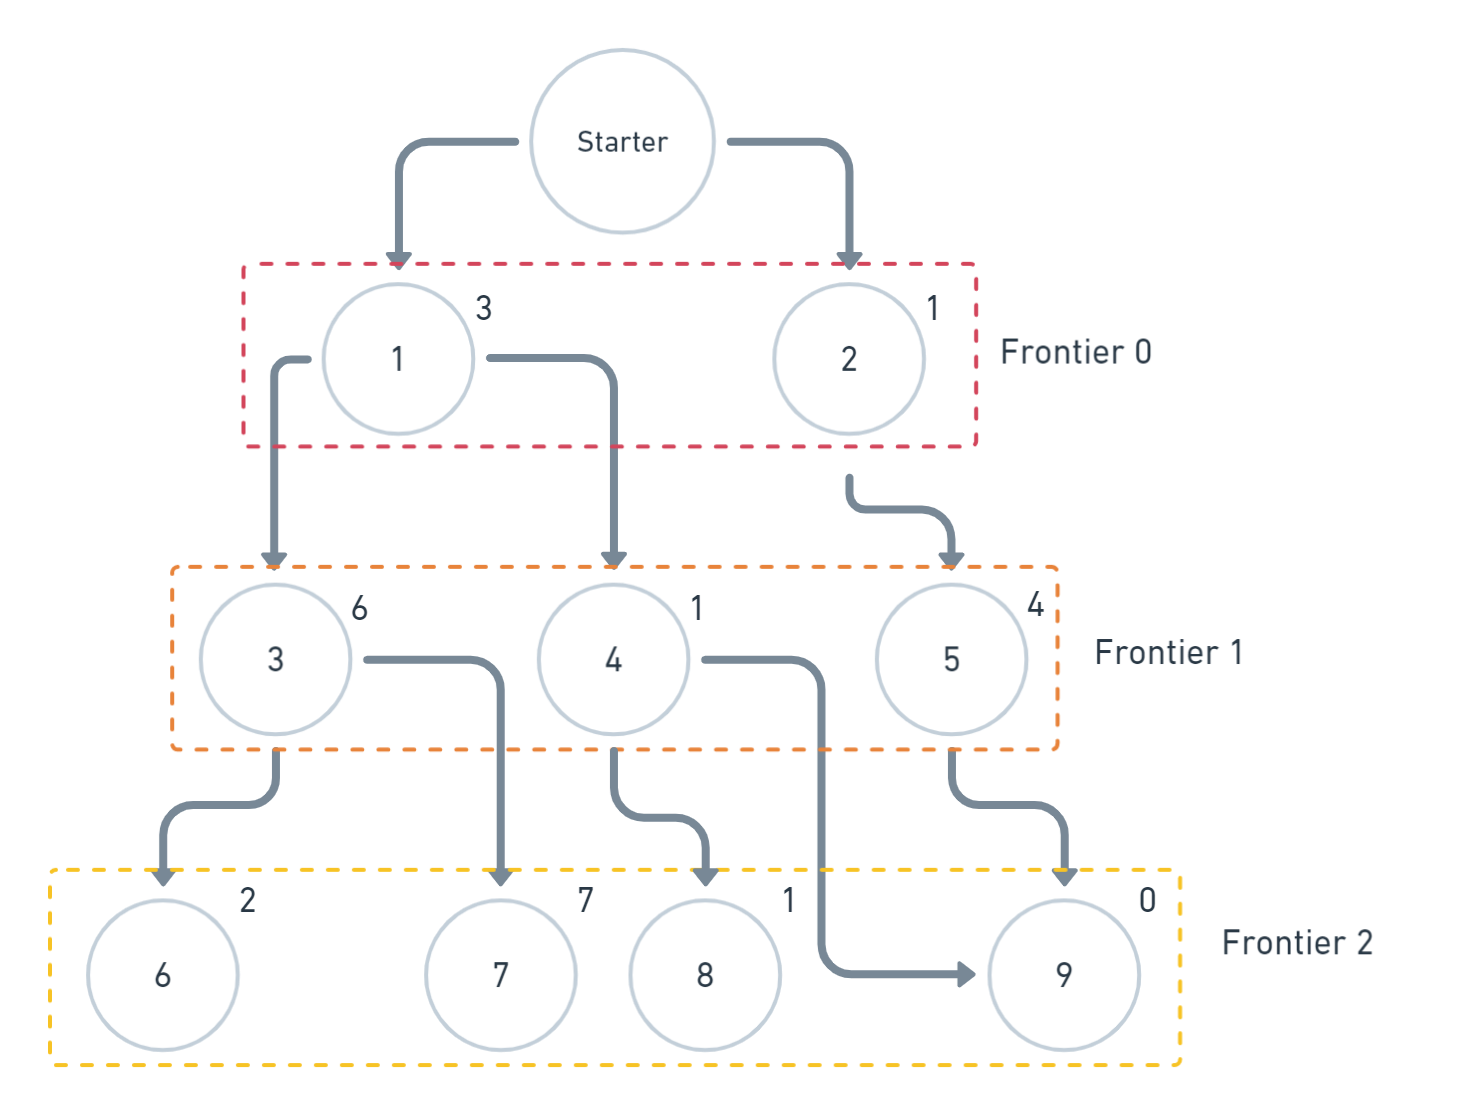
\includegraphics[width=0.58\textwidth]{Figures/seq_schema.png}
    \caption{Example of the BFS visit}
    \label{fig:bfs_tree}
\end{figure}
\FloatBarrier

\begin{figure}[htb!]
    \centering
    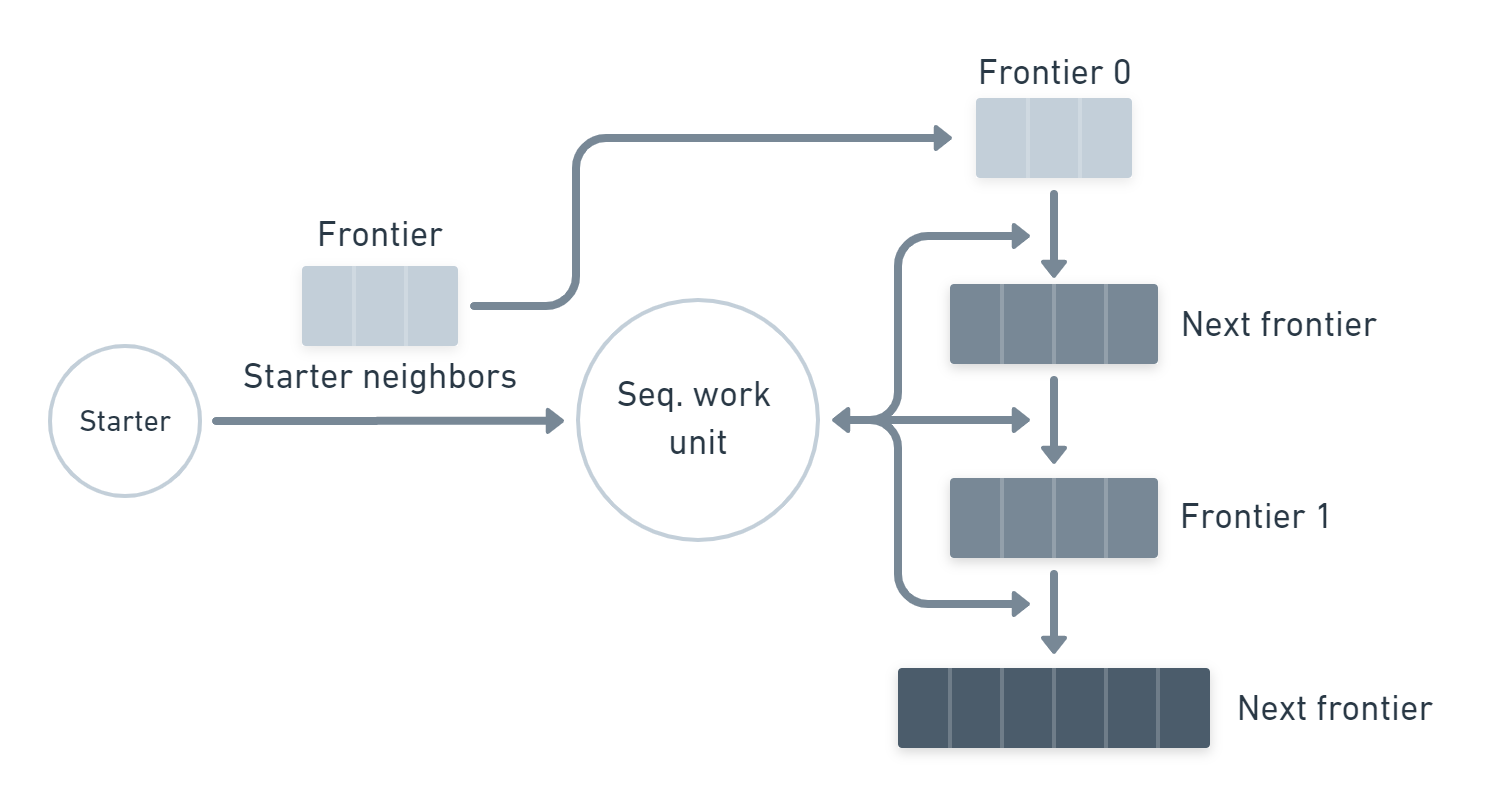
\includegraphics[width=0.8\textwidth]{Figures/seq_comp_schema.png}
    \caption{Schema of the sequential algorithm}
    \label{fig:bfs_seq_schema}
\end{figure}
\FloatBarrier

So in time terms the $BFS$ is performed as the sum (\ref{eq:T_seq}) of this two terms:

\begin{itemize}
    \item $T_{visit} (i)$ : as the time to visit a new i th frontier;
    \item $T_{swap}$: as the time to exchange the old with the new frontier.
\end{itemize}

\begin{equation}
\centering
T_{seq} = \displaystyle \sum_{i=0}^n T_{visit_i} + T_{swap}
\label{eq:T_seq}
\end{equation}

With $n$ as the number of frontiers and  $T_{visit_i} >>  T_{swap}$. Due to this last consideration the phase that lends itself best to be parallelized is frontier analysis. 
Considering to chose a farm-based approach and use $nw$ workers for visiting the frontier, we will obtain a visit time equal to $T_{visit}/nw$. However, to this, it is necessary to add the farm initialization time $T_{init}$, the time to divide and assign frontier chunks $T_e$ and the collecting time $T_c$. These last two terms replace the $T_{swap}$ of the sequential version.   
Thus the completion time of the parallel version will be:
\begin{equation}
\centering
T_{par} = T_{init} + \displaystyle \sum_{i=0}^n max\{T_e, T_{visit}/nw, T_c\}
\label{eq:T_par}
\end{equation}

It is necessary to say that everything depends on the properties of the graph, it makes sense to go for parallelization if you work with large frontiers in order to have $T_{visit}/nw >> T_{init} + T_e + T_c$. In fact, for graphs in which the degree of each node is very small, the disadvantages of parallelization will be greater than the benefits, this is due to the management of workers and synchronization in the merge phase of new frontiers. 

